\documentclass[en]{university}

\faculty{Department of Computer Engineering}
\course{Artificial Intelligence}
\subject{Mini Project 3 Theory Questions}
\professor{Dr. Rohban}
\student{Parsa Mohammadian}

\begin{document}

\setupdocument

\section{}

\subsection{}

We decide if a move violates game rules or not by using d-separation algroithm to find out 
if A and B are still independent. A valid move for each of the graphs is illustrated in 
figure \ref{fig:validmoves}.

\begin{figure}[!htbp]
    \centering
    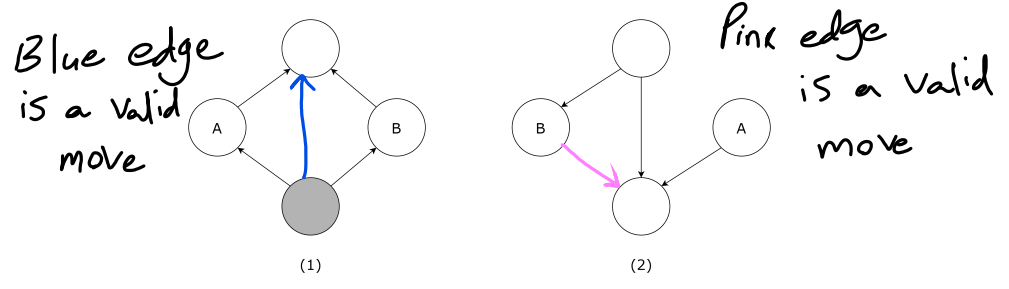
\includegraphics[width=0.8\textwidth]{assets/1-a.png}
    \caption{Valid Moves}
    \label{fig:validmoves}
\end{figure}

\subsection{}

In a tree structure, I propose a move for first player and consider every possible move for second player and evaluate outcome 
from the leaves. If I can find a tree with all win outcomes, then I find a win strategy for first player. 

First graph tree is shown in figure \ref{fig:tree1}. So this graph has a win strategy for first player.

Second graph tree is shown in figure \ref{fig:tree2}. So this graph has a win strategy for first player too.

\begin{figure}[!htbp]
    \centering
    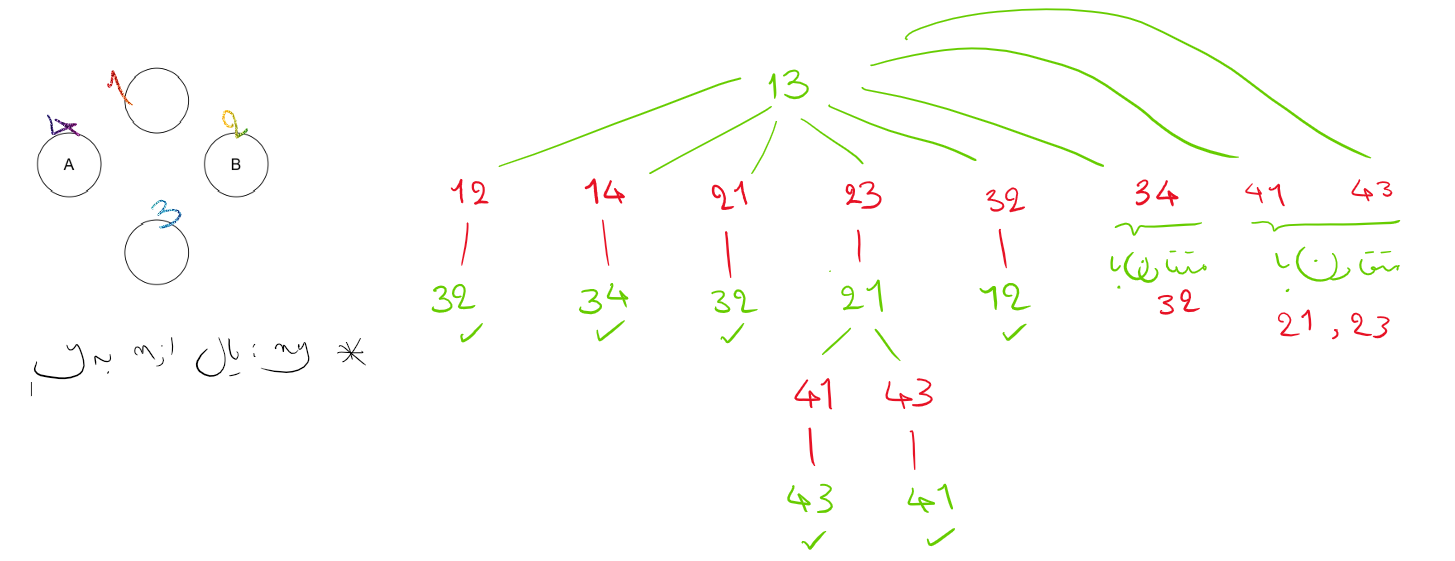
\includegraphics[width=\textwidth]{assets/1-b-1.png}
    \caption{First Graph Tree}
    \label{fig:tree1}
\end{figure}

\begin{figure}[!htbp]
    \centering
    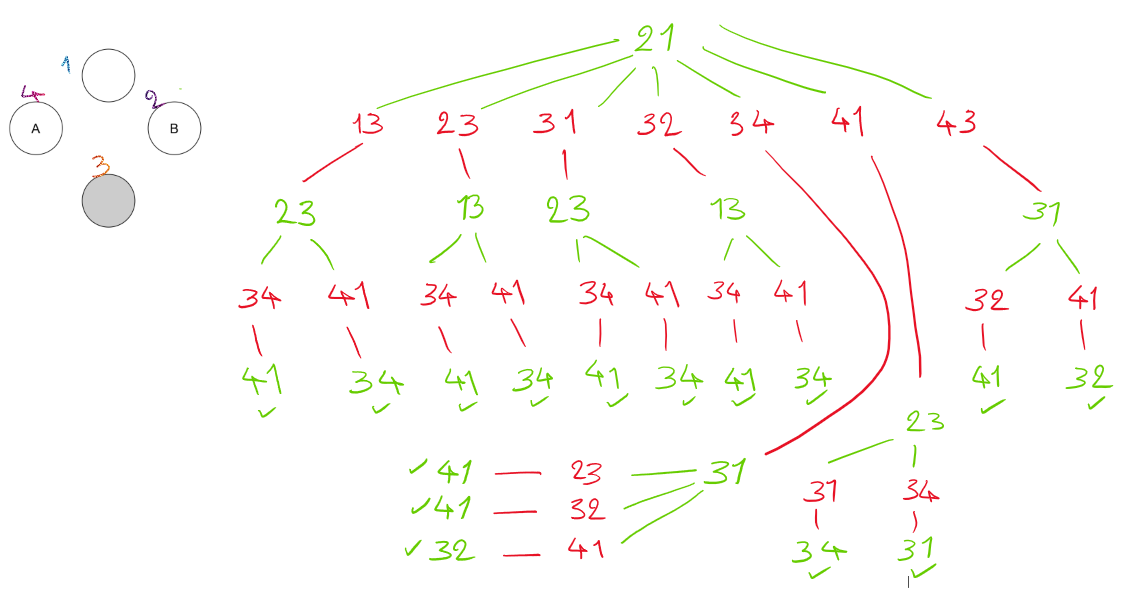
\includegraphics[width=\textwidth]{assets/1-b-2.png}
    \caption{Second Graph Tree}
    \label{fig:tree2}
\end{figure}

\section{}

Base factor headers are:

\begin{align*}
    A : \begin{bmatrix}
        A & C & D & P(A | C, D)
    \end{bmatrix} \\
    B : \begin{bmatrix}
        B & D & E & G & P(B | D, E, G)
    \end{bmatrix} \\
    C : \begin{bmatrix}
        C & F & I & P(C | F, I)
    \end{bmatrix} \\
    D : \begin{bmatrix}
        D & G & H & P(D | G, H)
    \end{bmatrix} \\
    E : \begin{bmatrix}
        E & P(E)
    \end{bmatrix} \\
    F : \begin{bmatrix}
        F & H & P(F | H)
    \end{bmatrix} \\
    G : \begin{bmatrix}
        G & H & P(G | H)
    \end{bmatrix} \\
    H : \begin{bmatrix}
        H & I & P(H | I)
    \end{bmatrix} \\
    I : \begin{bmatrix}
        I & P(I)
    \end{bmatrix}
\end{align*}

\subsection{B, E, D, C, H, I}

\begin{align*}
    f_1 = \text{Join} (B) \rightarrow \text{Eliminate} (B) : \begin{bmatrix}
        D & E & G & P(D, E, G)
    \end{bmatrix} \\
    f_2 = \text{Join} (f_1, E) \rightarrow \text{Eliminate} (E) : \begin{bmatrix}
        D & G & P(D, G)
    \end{bmatrix} \\
    f_3 = \text{Join} (f_2, A, D) \rightarrow \text{Eliminate} (D) : \begin{bmatrix}
        A & C & G & H & P(A, C, G, H)
    \end{bmatrix} \\
    f_4 = \text{Join} (f_3, C) \rightarrow \text{Eliminate} (C) : \begin{bmatrix}
        A & G & H & F & I & P(A, G, H, F, I)
    \end{bmatrix} \\
    f_5 = \text{Join} (f_4, F, G, H) \rightarrow \text{Eliminate} (H) : \begin{bmatrix}
        A & F & G & I & P(A, F, G, I)
    \end{bmatrix} \\
    f_6 = \text{Join} (f_4, I) \rightarrow \text{Eliminate} (I) : \begin{bmatrix}
        A & G & F & P(A, G, F)
    \end{bmatrix}
\end{align*}

\subsection{I, H, C, D, E, B}

\begin{align*}
    f_1 = \text{Join} (C, H, I) \rightarrow \text{Eliminate} (I) : \begin{bmatrix}
        C & F & H & P(C, F, H)
    \end{bmatrix} \\
    f_2 = \text{Join} (f_1, D, F, G) \rightarrow \text{Eliminate} (H) : \begin{bmatrix}
        C & F & D & G & P(C, F, D, G)
    \end{bmatrix} \\
    f_3 = \text{Join} (f_2, A) \rightarrow \text{Eliminate} (C) : \begin{bmatrix}
        A & D & F & G & P(A, D, F, G)
    \end{bmatrix} \\
    f_4 = \text{Join} (f_3, B) \rightarrow \text{Eliminate} (D) : \begin{bmatrix}
        A & F & G & B & E & P(A, F, G, B, E)
    \end{bmatrix} \\
    f_5 = \text{Join} (f_4, E) \rightarrow \text{Eliminate} (E) : \begin{bmatrix}
        A & F & G & B & P(A, F, G, B)
    \end{bmatrix} \\
    f_6 = \text{Join} (f_4) \rightarrow \text{Eliminate} (B) : \begin{bmatrix}
        A & F & G & P(A, F, G)
    \end{bmatrix}
\end{align*}

\subsection{Comparison}

The maximum size of the factor is $2^3$ for both orderings (Consider we know $F, G$). So we should compare each factor size. If we ignore evidence variables which we already 
know their values, clearly the second order is better one and need less time to be computed.

\section{}

\subsection{}

\begin{gather*}
    T : \text{Today} \\
    Y : \text{Yesterday} \\
    P(T = D) = P(T = D | Y = D) \times P(Y = D) \\ + P(T = D | Y = N) \times P(Y = N) \\
    \text{$Y$ and $T$ have the same distribution} \\
    \Rightarrow P(T = D) = 0.3 \times P(T = D) + 0.1 \times P(T = N) \\
    P(T = N) = 1 - P(T = D) \\
    \Rightarrow P(T = D) = 0.3 \times P(T = D) + 0.1 \times (1 - P(T = D)) \\
    = 0.3 \times P(T = D) + 0.1 - 0.1 \times P(T = D) \\
    = 0.2 \times P(T = D) + 0.1 \\
    \Rightarrow 0.8 \times P(T = D) = 0.1 \Rightarrow P(T = D) = \frac{0.1}{0.8} = 0.125 \\
\end{gather*}

\subsection{}

\begin{gather*}
    P(X = x | Dizinnes, Shortness of Breath) \\ \propto P(X = x, Dizinnes, Shortness of Breath) \\
    = \sum_{y} P(X = x) \times P(Shortness of Breath | X = x) \\ \times P(Dizinnes | Y) \times P(Y | X = x) \\
    \Rightarrow P(X = x | Dizinnes, Shortness of Breath) \\ = \frac{P(X = x, Dizinnes, Shortness of Breath)}{\sum_{x} P(X = x, Dizinnes, Shortness of Breath)} \\
    \Rightarrow P(X = Sepsis, Dizinnes, Shortness of Breath) \\ = 0.003 \times 0.85 \times 0.8 \times 0.7 + 0.003 \times 0.85 \times 0.7 \times 0.5 = 0.0023205 \\
    \Rightarrow P(X = Heart Muscle Weakness, Dizinnes, Shortness of Breath) \\ = 0.02 \times 0.5 \times 0.8 \times 0.7 + 0.02 \times 0.5 \times 0.7 \times 0.1 = 0.0063 \\
    \Rightarrow P(X = Sepsis | Dizinnes, Shortness of Breath) \\ = \frac{0.0023205}{0.0023205 + 0.0063} = 0.26918392204628505 \\
    \Rightarrow P(X = Heart Muscle Weakness | Dizinnes, Shortness of Breath) \\ = \frac{0.0063}{0.0023205 + 0.0063} = 0.7308160779537151
\end{gather*}

So the patient is more likely to have Heart Muscle Weakness.

\end{document}